% Lecture Template for ME3001-001-Tristan Hill - Spring 2017 - Fall 2017
% 
% Mechanical Engineering Analysis with MATLAB
%
% Systems of Linear Equations - Lecture 4
%


% Document settings
\documentclass[11pt]{article}
\usepackage[margin=1in]{geometry}
\usepackage[pdftex]{graphicx}
\usepackage{multirow}
\usepackage{setspace}
\usepackage{hyperref}
\usepackage{color,soul}
\usepackage{fancyvrb}
\usepackage{framed}
\usepackage{wasysym}
\usepackage{multicol}
\usepackage{amssymb}

\pagestyle{plain}
\setlength\parindent{0pt}
\hypersetup{
    bookmarks=true,         % show bookmarks bar?
    unicode=false,          % non-Latin characters in Acrobat’s bookmarks
    pdftoolbar=true,        % show Acrobat’s toolbar?
    pdfmenubar=true,        % show Acrobat’s menu?
    pdffitwindow=false,     % window fit to page when opened
    pdfstartview={FitH},    % fits the width of the page to the window
    pdftitle={My title},    % title
    pdfauthor={Author},     % author
    pdfsubject={Subject},   % subject of the document
    pdfcreator={Creator},   % creator of the document
    pdfproducer={Producer}, % producer of the document
    pdfkeywords={keyword1} {key2} {key3}, % list of keywords
    pdfnewwindow=true,      % links in new window
    colorlinks=true,       % false: boxed links; true: colored links
    linkcolor=red,          % color of internal links (change box color with linkbordercolor)
    citecolor=green,        % color of links to bibliography
    filecolor=magenta,      % color of file links
    urlcolor=blue           % color of external links
}

% assignment number 
\newcommand{\NUM}{3} 
\newcommand{\VSpaceSize}{2mm} 
\newcommand{\HSpaceSize}{2mm} 

%\definecolor{mygray}{rgb}{.6, .6, .6}
%\definecolor{mypurple}{rgb}{0.6,0.1961,0.8}
\definecolor{mygreen}{rgb}{0.1333 ,  0.5451,    0.1333}
\definecolor{mypink}{rgb}{0.1333 ,  0.5451,    0.1333}
\setulcolor{red} 
\setstcolor{green} 
\sethlcolor{mygray} 

\definecolor{mygreen}{rgb}{0, .39, 0}

%\definecolor{dred}{#8B0000}
% [153,50,204] - dark orchid
\definecolor{mypurple}{rgb}{0.6,0.1961,0.8}
%[139,69,19] - saddle brown
\definecolor{mybrown}{rgb}{0.5451,0.2706,0.0745}

\definecolor{mygray}{rgb}{.6, .6, .6}

\setulcolor{red} 
\setstcolor{green} 
\sethlcolor{mygray} 

\newcommand{\VA}{\vspace{2mm}}
\newcommand{\VB}{\vspace{5mm}} 
\newcommand{\VC}{\vspace{30mm}} 
 
\newcommand{\R}{\color{red}}
\newcommand{\B}{\color{blue}}
\newcommand{\K}{\color{black}}
\newcommand{\G}{\color{mygreen}}
\newcommand{\PR}{\color{mypurple}}

\begin{document}

\textbf{ \LARGE ME 3001 Lecture - Systems of Linear Equations} \\\\
\textbf{ \LARGE Potential Problems with Gaussian Elimination } \\


 \renewcommand\labelitemi{\textbullet}
 \renewcommand\labelitemii{\textendash}
 \renewcommand\labelitemiii{\textasteriskcentered}
 \renewcommand\labelitemiv{\textperiodcentered}

\Large
\begin{itemize}

\item \textbf{  Remember, our motivation is to develop a {\B General Method} to solve this type of problem. Meaning I want my solution work for any problem of the {\PR standard form}.} \\\\

\scalebox{1.2}{$	 	
 \left( \begin{array}{cccc}
a_{11} & a_{12} & ...& a_{1n} \\
a_{21} & a_{22} & ...& a_{2n} \\
&.&&\\
&.&&\\
a_{n1} & a_{n2} & ...& a_{nn}\end{array} \right) \times \left[ \begin{array}{c}
x_1 \\
x_2 \\
.\\
.\\
x_n \end{array} \right] = \left[ \begin{array}{c}
b_1 \\
b_2 \\
.\\
.\\
b_n \end{array} \right] 
$}\\\\

\hspace*{15mm}\scalebox{2}{$[ A ] \times \vec{x}  = \vec{b} $} \\\\


\item \textbf{  There are several errors that may occur} \\
	\begin{itemize}
		\item \textbf{ we obviously must follow the rules of mathematics}\vspace{20mm}\\
	
		\item \textbf{ some problems or systems are not solvable} \vspace{20mm}\\
		\item \textbf{ we want to have the least error with the least work}
	\end{itemize}
\newpage


\Large
\item \textbf{ What is 1 thing that you cannot do math???} \\

	\begin{itemize}
		\item \scalebox{1.2}{$	 	
 \left( \begin{array}{cccc}
a_{11} & a_{12} & ...& a_{1n} \\
a_{21} & a_{22} & ...& a_{2n} \\
&.&&\\
&.&&\\
a_{n1} & a_{n2} & ...& a_{nn}\end{array} \right) \times \left[ \begin{array}{c}
x_1 \\
x_2 \\
.\\
.\\
x_n \end{array} \right] = \left[ \begin{array}{c}
b_1 \\
b_2 \\
.\\
.\\
b_n \end{array} \right] 
$}\\\\

	\item \textbf{ the {\it diagonal elements} are called {\it pivot elements} or sometimes just {\it pivots}}\\
	\item \textbf{ take a look back at the algorithm one more time} \\\\
	\scalebox{1.3}{ {\it for} \color{mypurple}k \color{black} {\it from} 1 {\it to} \color{mygreen}n\color{black}-1} \\
	
		\hspace{10mm} \scalebox{1.3}{{\it for} \color{blue}i \color{black} {\it from} \color{mypurple}k\color{black}+1 {\it to} \color{mygreen}n\color{black}} \\
		
		\hspace{20mm} \scalebox{1.3}{fact$=a_{\color{blue}i\color{black},\color{mypurple}k}/a_{\color{mypurple}k\color{black},\color{mypurple}k\color{black}}$} \\

		\hspace{20mm} \scalebox{1.3}{{\it for} \color{red}j \color{black} {\it from} \color{mypurple} k \color{black}  {\it to} \color{mygreen}n\color{black}}\\

		\hspace{30mm} \scalebox{1.3}{$a_{\color{blue}i\color{black},\color{red}j}=a_{\color{blue}i\color{black},\color{red}j}-$fact$\times a_{\color{mypurple}k\color{black},\color{red}j}$}\\
\hspace*{20mm}\scalebox{1.3}{{\it end}}\\
\hspace*{20mm}\scalebox{1.3}{$b_{\color{blue}i\color{black}}=b_{\color{blue}i\color{black}}-$fact$\times b_{\color{mypurple}k\color{black}}$}\\
\hspace*{10mm}\scalebox{1.3}{{\it end}}\\ 	
\scalebox{1.3}{{\it end}}\\ 	 

	\item \textbf{ how can we avoid this problem?}

\newpage
	\item \textbf{to avoid this issue we can use the tools we have and they are ...}\\

	\item \textbf{\scalebox{1.5}{Elementary Row Operations}}\\
	\begin{itemize}
		\item \textbf{Row Switching}\vspace{15mm}\\ 
		\item \textbf{Row Multiplication}\vspace{15mm}\\ 
		\item \textbf{Row Addition}\vspace{15mm}\\ 
	\end{itemize}
	
	\item \textbf{the act of avoiding this error is called  \PR \scalebox{2}{{\it pivoting}} \K}\\
	\begin{itemize}
		\item \textbf{Partial Pivoting}\vspace{8mm}\\ 
		\item \textbf{Scaled Partial Pivoting}\vspace{8mm}\\ 
		\item \textbf{Complete Pivoting}\vspace{8mm}\\ 
		\item \textbf{Virtual Pivoting}\vspace{8mm}\\ 
		\item \textbf{No Pivoting - Naive Gaussian Elimination}
	\end{itemize}
	
	
	\item \textbf{Partial Pivoting Example}\\
	\vspace{100mm}
	\end{itemize}
%	\newpage
%\Large
%\item \textbf{ We also want our answer to have as little \scalebox{1.5}{error} as possible} \\
%	\begin{itemize}
%		\item \textbf{What causes error in the numerical methods?} \\
%			``In software engineering and mathematics, numerical error is the combined effect of two kinds of error in a calculation. The first is caused by the finite precision of computations involving floating-point or integer values. The second usually called truncation error is the difference between the exact mathematical solution and the approximate solution obtained when simplifications are made to the mathematical equations to make them more amenable to calculation.''-wikipedia\\
%		\item \textbf{2 (or 3) Major Causes} \\
%			\begin{itemize}
%				\item \textbf{floating point computations} \vspace{20mm}\\
%				\item \textbf{truncation and solution simplification} \vspace{20mm}\\
%				\item \textbf{system condition} \vspace{20mm}\\
%			\end{itemize}
%	\end{itemize}
	
	\newpage
\Large
\item \textbf{ Some problems cannot be solved with this type of technique!} \\	
\begin{itemize}
\item {\PR non-homogeneous} system is one in which ... \vspace{10mm}\\
\item most of the time the system will be {\PR non-homogeneous} \vspace{10mm}\\
\item a {\PR non-homogeneous} system has a {\B proper solution} if and only if ...\vspace{10mm}\\
	
	\scalebox{2}{$rank(A)=rank([A | b])=n$}

\newpage
\item {\bf Normal Case - 2 Equations - 2 Unknowns - 1 Solution} \\\\ 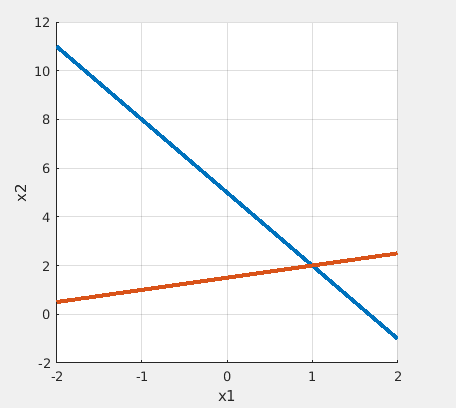
\includegraphics[scale=1]{lecture4_fig1.png} \\\\
\scalebox{2}{$3x_1+x_2=5$}\\\\
\scalebox{2}{$x_1-2x_2=-3$}

\newpage
\item {\bf Abnormal Case - 2 Equations - 2 Unknowns - $\infty$ Solutions} \\\\ 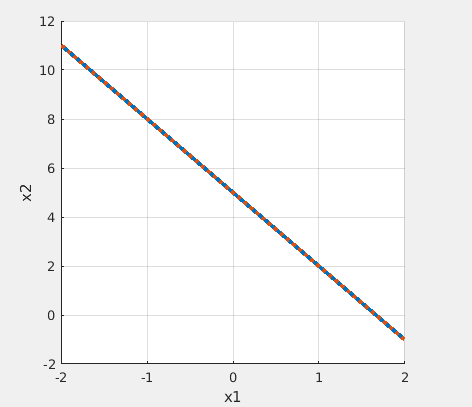
\includegraphics[scale=1]{lecture4_fig2.png} \\\\
\scalebox{2}{$3x_1+x_2=5$}\\\\
\scalebox{2}{$6x_1+2x_2=10$}

\newpage
\item {\bf Abnormal Case - 2 Equations - 2 Unknowns - 0 Solutions} \\\\ 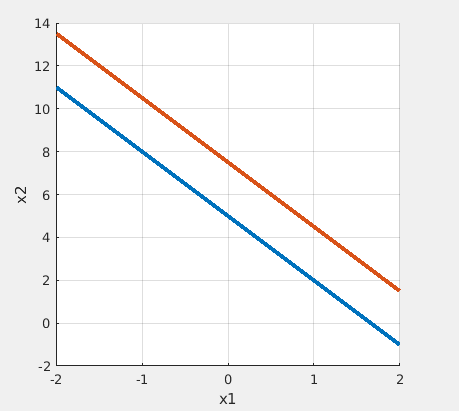
\includegraphics[scale=1]{lecture4_fig3.png} \\\\
\scalebox{2}{$3x_1+x_2=5$}\\\\
\scalebox{2}{$6x_1+2x_2=15$}

\newpage
\item {\bf Abnormal Case - 3 Equations - 2 Unknowns - 0 Solutions} \\\\ 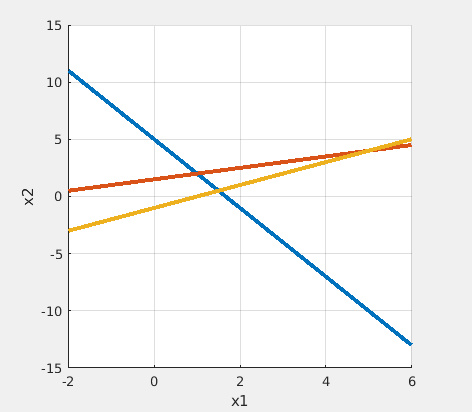
\includegraphics[scale=1]{lecture4_fig4.png} \\\\
\scalebox{2}{$3x_1+x_2=5$}\\\\
\scalebox{2}{$x_1-2x_2=-3$}\\\\
\scalebox{2}{$x_1-x_2=1$}

\newpage
\item {\bf Abnormal Case - 3 Equations - 2 Unknowns - 1 Solution} \\\\ 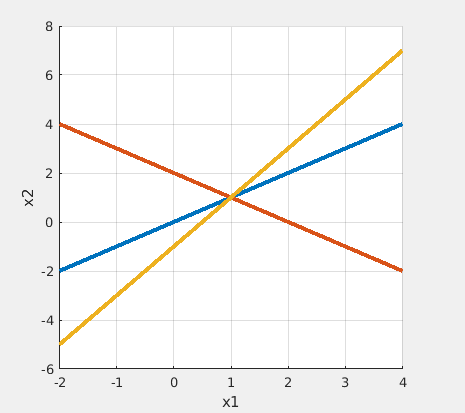
\includegraphics[scale=1]{lecture4_fig5.png} \\\\
\scalebox{2}{$-x_1+x_2=0$}\\\\
\scalebox{2}{$x_1+x_2=2$}\\\\
\scalebox{2}{$-2x_1+x_2=-1$}
\end{itemize}


\newpage 
\newpage
\Large
\item \textbf{ We also want our answer to have as little \scalebox{1.5}{error} as possible} \\
	\begin{itemize}
		\item \textbf{What causes error in the numerical methods?} \\
			``In software engineering and mathematics, numerical error is the combined effect of two kinds of error in a calculation. The first is caused by the finite precision of computations involving floating-point or integer values. The second usually called truncation error is the difference between the exact mathematical solution and the approximate solution obtained when simplifications are made to the mathematical equations to make them more amenable to calculation.''-wikipedia\\
		\item \textbf{2 (or 3) Major Causes} \\
			\begin{itemize}
				\item \textbf{floating point computations} \vspace{20mm}\\
				\item \textbf{truncation and solution simplification} \vspace{20mm}\\
				\item \textbf{system condition} \vspace{20mm}\\
			\end{itemize}
	\end{itemize}

\newpage
\item \textbf{ The {\B System Condition} can cause problems!} \\
\begin{itemize}
	\item An {\PR ill-conditioned} system can cause error. \\\\
	
	\item A system is {\PR ill-conditioned} if small changes in the coefficients on the either side of the equation create large variations in the solution.\\\\

	\item Let us look at a simple 2x2 example. \\\\
	
		\scalebox{1.5}{$x_1 - x_2=5$} \\\\
		\scalebox{1.5}{$kx_1 - x_2=4$}\\\\
	
	\item The system shown will have huge variations in the solution if \scalebox{1.5}{$k\approx 1$}\\\\
	
		\scalebox{1.5}{$x_1 - x_2=5$} \\\\
		\scalebox{1.5}{$(0.99)x_1 - x_2=4$}\\\\
	\item When \scalebox{1.5}{$k = 0.99$}, this gives a solution \scalebox{1.5}{$(x_1,x_2)=(100, 95)$}	\\\\
	
	\scalebox{1.5}{$x_1 - x_2=5$} \\\\
		\scalebox{1.5}{$(1.01)x_1 - x_2=4$}\\\\
	\item When \scalebox{1.5}{$k = 1.01$}, this gives a solution \scalebox{1.5}{$(x_1,x_2)=(-100, 105)$}	

\end{itemize}
\newpage 

	 \item \textbf{ \LARGE REMINDER - Homework 2 is due now due on Friday !} \\
 \item \textbf{ \LARGE REMINDER -Exam1 is coming up!} \\
\end{itemize}


	

\end{document}



